%!TEX root = practicum1.tex
\todo[inline]{Check referenties}
\todo[inline]{Nalezen}

We perform two different experiments with the Chirikov map defined in \cref{eq:chirikov}. In \cref{ss:fixed} we fix the value of the non-linearity parameter and explore the influences of different values for $p_0$ and $x_0$. In \cref{ss:variable} we discuss the influence of the non-linearity parameter $K$. Plotting various Chirikov maps with randomly chosen initial conditions for $K = 1$ results in decorative images, such as the one presented in \cref{fig:a:pretty}.

	\begin{figure}[b]
		\centering
		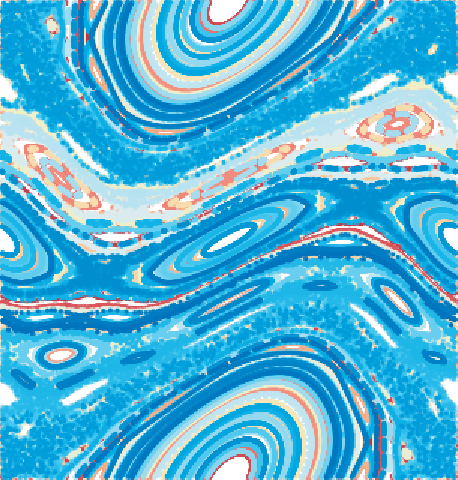
\includegraphics[width=0.9\columnwidth]{./img/assignment_a_pretty_low_res.pdf}
		\caption{500 randomly initialized orbits of the Frenkel-Kontorova model for $K = 1$.}
		\label{fig:a:pretty}
	\end{figure}

\subsection[]{Fixed $K$}
\label{ss:fixed}
%!TEX root = practicum1.tex
We have fixed the value of $K$ to 1, essentially removing the parameter from the equation. By choosing different initial values we can generate three different kinds: zero-, one and two-dimensional, these different orbits are discussed in respectively \cref{sss:experiment:a:discrete}, \ref{sss:experiment:a:closed} and \ref{sss:experiment:a:2D}.

 	\begin{figure}
		\centering
		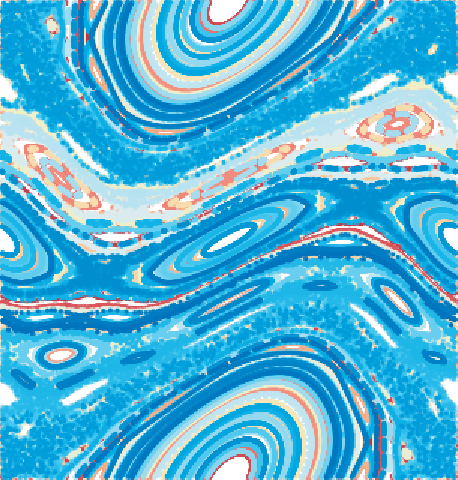
\includegraphics[width=0.9\columnwidth, height=0.2\textheight, keepaspectratio=true]{./img/assignment_a_pretty_low_res.pdf}
		\caption{Phase-space diagram, $p_n$ as a function of $x_n$, of 500 randomly initialized orbits of the Frenkel-Kontorova model for $K = 1$, with $0 \leq n \leq 1000$, and $x_0$ and $p_0$ in the unit square.}
		\label{fig:a:pretty}
	\end{figure}

\subsubsection{Discrete Points}
\label{sss:experiment:a:discrete}
Zero-dimensional orbits consist of a finite number of points, which are found in the centers of the islands in \cref{fig:a:pretty} \cite{kenzel1997physics}. 

We have generated a one-dimensional Chirikov map by choosing $x_0 = p_0 = 0.5$. Using these values $p_1 = p_0$ since the second term of \eqref{eq:chirikov:p} becomes zero. This results in $x_1 = \left( x_0 + p_{1} \right) \mod 1= 0$. The next steps are easily derived since $p_{n + 1}$ for $n > 0$ will not change due to the fact that both 0 and 0.5 as input to \eqref{eq:chirikov:p} will result in the second term becoming zero. With this initialization $x_{n} \in \left\{0,\, 0.5 \right\} \text{ for } n \geq 0$. To illustrate $x_2$ is $0.5 + 0 = 0.5$ which is equal to $x_1$. We have now shown that $p_n$ is constant for $n \geq 1$ and that $x_n$ jumps between 0 and 0.5, which is illustrated in \cref{fig:experiment:dimension:0:t}. This conclusion also explains the results in \cref{fig:experiment:dimension:0}. 

Furthermore we have shown that these points are visited in a fixed order, which explains the plots in \crefrange{fig:experiment:dimension:0:x}{fig:experiment:dimension:0:p}.\\

From this specific case we can derive the following constraints for $p_0$ and $x_0$; $x_0$ should be chosen in such a way that the sine in \cref{eq:chirikov:p} becomes 0, i.e. $x_0 \in \{0,\, 0.5,\, 1\}$. Due to the constraint on $x_0$,
\begin{equation*}
p_{n + 1} = p_{n} \mod 1,
\end{equation*}
	which is equal to $p_n$, unless $p_n = 1$. Consequently
	\begin{equation*}
	x_{n + 1} = x_n + p_n \mod 1,
	\end{equation*}
unless $p_1 = 1$. Formally, one should choose $p_0$ in such a way that:
\begin{equation*}
	\left( \left[ x_0 + (p_0 \mod 1)\right] \mod 1 \right) \in \left\{0, 0.5, 1\right\}.
\end{equation*}

\subsubsection{Closed curves}
\label{sss:experiment:a:closed}
One dimensional orbits are represented in the phase-space diagram in \cref{fig:a:pretty} as the closed curves around the islands formed by the zero-dimensional orbits.

We have determined empirically that $\left\{x_0\,, p_0 \right\} = {\num{0.1576131},\,\num{0.9705928}}$ results in closed curves. \Cref{fig:experiment:dimension:1} shows $p_n$ as a function of $x_n$, \crefrange{fig:experiment:dimension:1:x}{fig:experiment:dimension:1:p} shows the progression of respectively $p$ and $x$.\\

Considering these figures we see that the progression of both $p$ and $x$ happens according to a fixed pattern with a seemingly periodic shift. Examining \cref{fig:experiment:dimension:1:t} we see that $x$, the orange dashed points, slowly moves from one extreme to the other, which is reflected in \cref{fig:experiment:dimension:1:x}. Considering $p$ in \cref{fig:experiment:dimension:1:t}, the solid blue line, we find that its value moves between approximately 0.2 and 0.8, and then oscillates around that value before going back to the other value. This is represented in \cref{fig:experiment:dimension:1:p} by the high density areas in the lower left and upper right corners.

\begin{figure}
	\centering
	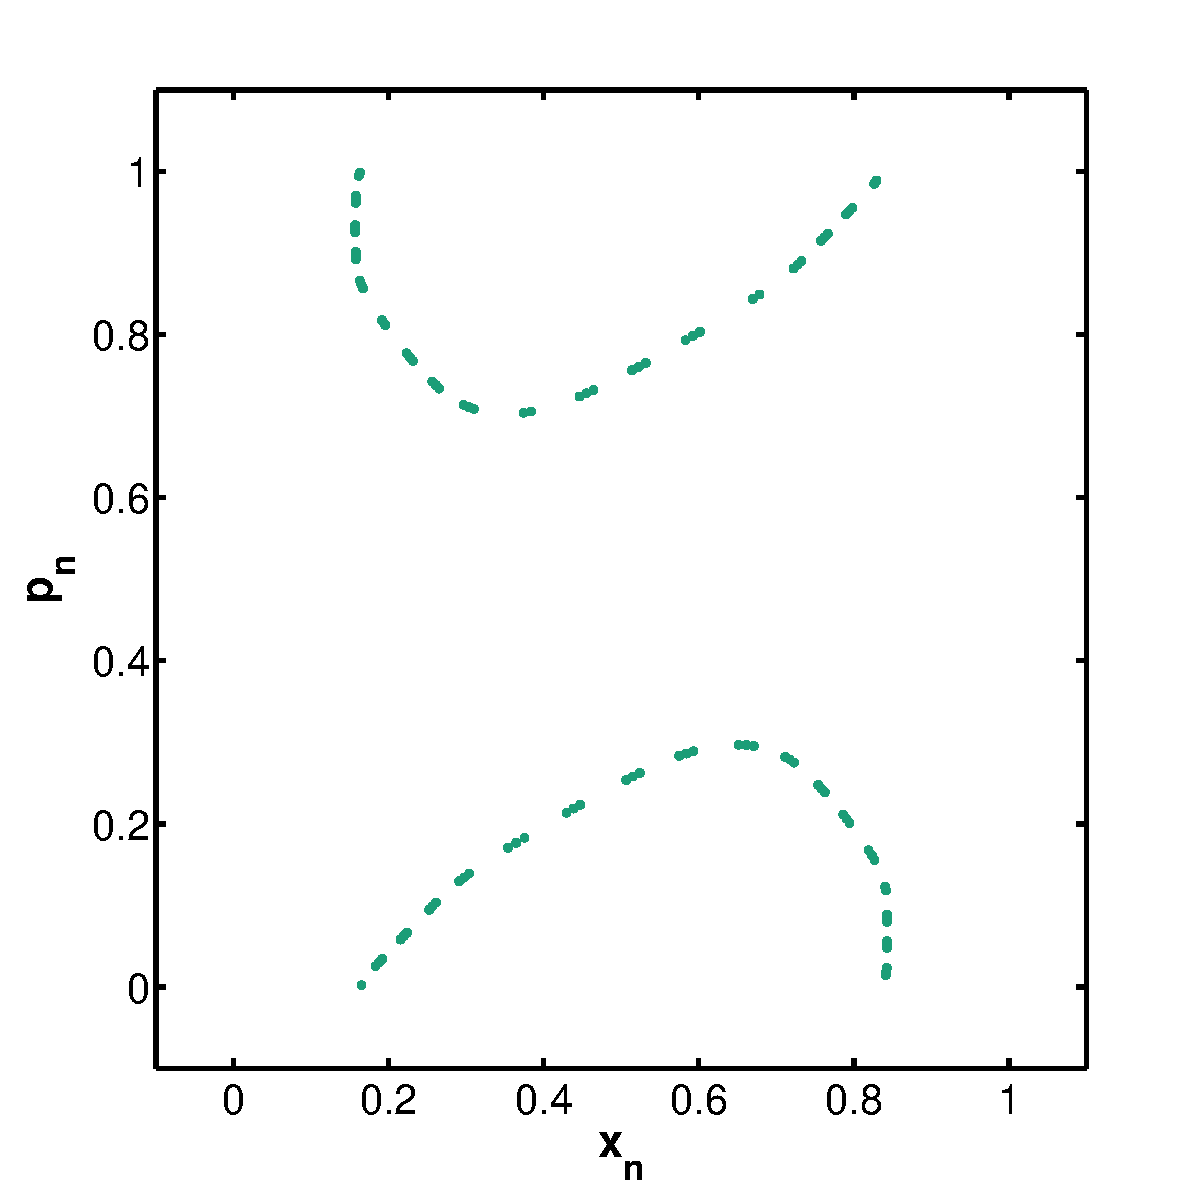
\includegraphics[width=0.9\columnwidth]{./img/assignment_a_1_dim_n100}
	\caption{$p_n = \num{0.1576131}$ as a function of $x_n= \num{0.9705928}$, for $n = 100$.}
	\label{fig:experiment:a_1_n100}
\end{figure}

%!TEX root = practicum1.tex

\begin{figure*}
	\centering
	% \x/\picname in {4/pic1.png,8/pic2.png,15/pic3.png,16/pic4.png}
	\foreach \dim/\x/\p in {0/0.500/0.500, 1/0.1576131/0.9705928, 2/0.1269868/0.9133759}
	{ 
		\begin{subfigure}[t]{0.32\textwidth}
			\includegraphics[width=\textwidth]{./img/assignment_a_\dim_dim.pdf}
			\caption{$x_0=\num{\x}$, $p_0=\num{\p}$}
			\label{fig:experiment:dimension:\dim}
		\end{subfigure}
		\begin{subfigure}[t]{0.32\textwidth}
			\includegraphics[width=\textwidth]{./img/assignment_a_\dim_dim_progression_p.pdf}
			\caption{Progression of $p$ in \subref{fig:experiment:dimension:\dim}}
			\label{fig:experiment:dimension:\dim:x}
		\end{subfigure}		
		\begin{subfigure}[t]{0.32\textwidth}
			\includegraphics[width=\textwidth]{./img/assignment_a_\dim_dim_progression_x.pdf}
			\caption{Progression of $x$ in \subref{fig:experiment:dimension:\dim}}
			\label{fig:experiment:dimension:\dim:p}
		\end{subfigure}		
	}
	\caption{Each row corresponds to on set of initial values $\left\langle x_0, p_0 \right\rangle$. The first column shows $x_n$ versus $p_n$ for $n \in \left[0,\, \num{10000} \right]$. The second and third column depict respectively the progression of $p$ and $x$.}
	\label{fig:experiment:dimension}
\end{figure*}

Thus we can conclude that the points of \cref{fig:experiment:dimension:1} are visited in a fixed order. Colloquially one could say that the map starts by generating a low density version of \cref{fig:experiment:dimension:1}, see \cref{fig:experiment:a_1_n100}, which is then filled in by iterating over the figure multiple times. Due to the small shift the area of the close curve is filled in after a large number of iterations.

\subsubsection{Two-Dimensional Orbits}	
\label{sss:experiment:a:2D}
	Two-dimensional orits fill entire areas by jumping around chaotically. The empirically determined values $\left\{x_0\,, p_0 \right\} = {\num{0.1269868},\,\num{0.9133759}}$ result in an orbit that fills the two-dimensional areas in \cref{fig:experiment:dimension:2}. Comparing \cref{fig:experiment:dimension:1:p} with \cref{fig:experiment:dimension:2:p} we see the same general pattern, however \cref{fig:experiment:dimension:2:p} shows more chaotic behaviour. We observe the same behaviour for $x$ when contrasting \cref{fig:experiment:dimension:1:x} with \cref{fig:experiment:dimension:2:x}. This is supported by comparing \cref{fig:experiment:dimension:1:t} with \cref{fig:experiment:dimension:2:t}, where we find that the blue and orange line have the same trajectory, approximately but that the lines in \cref{fig:experiment:dimension:2:t} change more, and change with a varying value every period.

	Since the map with orbits is essentially the same as the map with the closed curves the single points are also visited in a fixed order. 

	As the values of $p$ and $x$ vary more, we plotting $p$ as a function of $x$ results in an area around the curves that we saw in \cref{fig:experiment:dimension:1}.


\subsection[]{Variable $K$}
\label{ss:variable}
%!TEX root = practicum1.tex
The parameter $K$ defines how hard the system is driven, i.e. for $K = 0$ we would expect no perturbations, this case is discussed in \cref{ss:b:trivial}. As the value of $K$ increases we expect that the chaotic regions grow and eventually start to dominate the phase space \cite{finn200Cahaotic}. The effect of varying values of $K$ is discussed in \cref{ss:b:nontrivial}. Finally \cref{ss:b:kam} discusses KAM theory and how it relates to the Chirikov map. 

\subsection{Trivial Case}
\label{ss:b:trivial}
If we choose $K = 0$ \cref{eq:chirikov} becomes:
\begin{subequations}\label{eq:chirikovK0}
	\begin{align}
		\label{eq:chirikov0:p} p_{n + 1} &= p_n \mod 1,\\
		\label{eq:chirikov0:x} x_{n + 1} &= x_n + p_{n + 1} \mod 1.
	\end{align}
\end{subequations}	
Consequently the values of $p_n$ are constant for $n > 0$, since if $p_0 = 1$, $p_1 = 0$ as a consequence of the modulo operator in \eqref{eq:chirikov0:p}. Consequently without modulo 1, $x_n$ would increase linearly, due to this operator $x_n$ is periodic. 

\Cref{fig:experiment:K0influenceOfX} shows $x_0$ as a function of $n$ for a fixed value of $p_0$, if we compare the different plots  in this figure we observe that changing $x_0$ and fixing $p_0$ only influences the phase of $x_n$, and not the period. 

\begin{figure}
	\centering
	\foreach \x/\actualX in {1/0.1, 3/0.3, 5/0.5}{
		\begin{subfigure}[t]{\columnwidth}
			\includegraphics[width=\textwidth]{./img/assignment_b_K=0p_0=04x_0=0\x.pdf}
			\caption{$x_0 = \actualX$}
			\label{fig:experiment:K0:X:\x}
		\end{subfigure}	
	}	
	\caption{$x_n$ as a function of $n$, for $p_0 = 0.4$ and varying $x$.}
	\label{fig:experiment:K0influenceOfX}
\end{figure}

Fixing $x_0$ and varying $p_0$ results in \cref{fig:experiment:K0influenceOfP}, these plots show that $p_0$ influences the periodicity of the map, that is increasing $p_0$, increases the frequency.

\begin{figure}
	\centering
	\foreach \p/\actualP in {1/0.1, 3/0.3, 5/0.5}{
		\begin{subfigure}[t]{\columnwidth}
			\includegraphics[width=\textwidth]{./img/assignment_b_K=0p_0=0\p x_0=04.pdf}
			\caption{$p_0 = \actualP$}
			\label{fig:experiment:K0:P:\p}
		\end{subfigure}	
	}	
	\caption{$x_n$ as a function of $n$, for $x_0 = 0.4$ and varying $p$.}
	\label{fig:experiment:K0influenceOfP}
\end{figure}

\begin{figure*}
	\centering
	\foreach \k/\fnk in {0/0, 0.2/2, 0.4/4, 0.8/8, 1/10, 2/20, 3/30, 4/40}{
		\begin{subfigure}{0.24\textwidth}
			\centering
			\includegraphics[width=\textwidth]{./img/assignment_b_fancy_k_\fnk.jpg}
			\caption{$K = \k$}
			\label{fig:experiment:fancy_k:\k}
		\end{subfigure}
	}
	\caption{Full 100 run chirikov maps, for different $K$. For each map 1000 iterations and random initialisation for $x_0$ and $p_0$ were used.}
	\label{fig:experiment:fancy_k}
\end{figure*}


\subsection{Non-Trivial Case}
\label{ss:b:nontrivial}
\todo[inline]{How do the orbits change with increasing K? Do we have scenarios that are similar to period doubling?}
\todo[inline]{Discuss similarities and differences to logistic map}

\subsection{KAM-orbits}
\label{ss:b:kam}
\todo[inline]{Refind $K_C$ in literatur and try to confirm that KAM orbits exist just below but not above $K_c$}